\section{Auswertung}

\subsection{Untersuchung der Filterkurve des Selektivverstärkers.}

Zunächst soll die Durchlassfrequenz des Selektivverstärkers bestimmt werden. Dafür wurde die Ausgangsspannung bei verschiedenen Frequenzen gemessen. Die Messwerte stehen in Tabelle \ref{tab:1}. Graphisch dargestellt wurden dies Messwerte in Abbildung \ref{fig:durchlass}. In Abbildung \ref{fig:durchlass} ist auch eine Ausgleichsgraph zu erkennen. Der Ausgleichsgraph wurde mit einer Gleichung der Form

\begin{equation} \label{Voigt}
    f(x) = \alpha \cdot exp \left( - \frac{(x-\beta)^2}{2\gamma^2} \right) + \frac{\delta}{1+\left(\frac{x-\epsilon}{\zeta}\right)^2}
\end{equation}

\begin{figure}
    \centering
    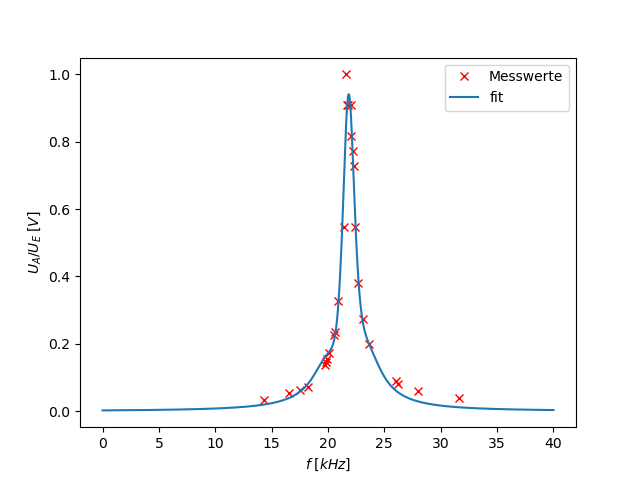
\includegraphics{durchlass.png}
    \captionof{figure}{Graphische Darstellung der Messwerte für die Bestimmung der Durchlassfrequenz des Selektivverstärkers.}
    \label{fig:durchlass}
\end{figure}

\noindent Die in der Formel \ref{Voigt} zu sehenden Konstanten wurden durch eine Ausgleichsrechnung mit dieser Formel bestimmt. Dabei entstehen für diese Konstanten folgende Werte

\begin{align*}
    \alpha &=   -0.605 \pm 0.224 \; V \\
    \beta &=   21.753 \pm 0.115 \; kHz \\
    \gamma &=    1.145 \pm 0.363 \; kHz \\
    \delta &=    1.544 \pm 0.228 \; V \\
    \epsilon &=   21.825 \pm 0.039 \; kHz \\
    \zeta &=    0.852 \pm 0.091 \; kHz. \\
\end{align*}

\noindent Mit $ f(x) = \frac{1}{\sqrt{2}} $ ergeben sich als Grenzen für die Breite die Werte $v_- = 20.89 \pm 0.03 \; kHz$ und $v_+ = 22.76 \pm 0.03 \; kHz$

\noindent Mit der Gleichung $Q = \frac{v_0}{v_+ - v_-}$ und $v_0 = \beta$ ergibt sich die Güte zu $Q = 11.63\pm 0.27$

\subsection{Bestimmung der Suszeptibilität von Oxiden einiger Erd-Elemente}

In diesem Versuchsteil wurden Spannungs- und Widerstandsdifferenzen einer Brückenschaltung mit zwei Spulen gemessen, wenn in die eine Spule eine Probe des jeweiligen Oxids eingeführt wird. Für die Berechnung der Suszeptibilität müssen noch Werte bestimmt werden. Das sind zum einen die realen Querschnitte der Proben. Diese können mit 

\begin{equation*}
    Q_\text{Real} = \frac{M_p}{L\cdot \rho_w}
\end{equation*}

\noindent berechnet werden wobei L die Länge, $\rho_w$ die Dichte und M$_p$ die molare Masse der Probe darstellt. 
Zum Anderen wird die Zahl der Momente pro Volumeneinheit N benötigt. Diese berechnet sich durch

\begin{equation*}
    N = 2 \cdot N_A \cdot \frac{\rho_w}{M_p}.
\end{equation*}

\noindent Dabei ist N$_A$ die Avogadrokonstante.

\subsubsection{Dysprosium}

Die Länge der Dysprosium-Probe beträgt 0.147m und ihre Masse beträgt 0.0151kg. 

\noindent Für die Dysprosium-Probe wurden die Werte in Tabelle \ref{tab:2} gemessen. Mit R$_3$ = 1000 $\Omega$, U$_{Sp}$ = 0.68 V und den Formeln \ref{XU} sowie \ref{XR} können die Suszeptibilitäten bestimmt werden. Die Werte lassen sich zu 

\begin{minipage}{\linewidth}
    \begin{table}[H]
        \centering
    \captionof{table}{Berechnete Suszeptibilitäten der Dysprosium-Probe.}
    \begin{tabular}{lll}
        \toprule
        Messung & $\chi_U$ & $\chi_R$ \\
        \midrule
        1 & 0.0438 & 0.0204 \\
        2 & 0.0431 & 0.0200 \\
        3 & 0.0421 & 0.0197 \\
        \midrule
        Mittelwerte & 0.043 & 0.02 \\
        \bottomrule   
    \end{tabular}
    
    \label{tab:4}
\end{table}
\end{minipage}

\subsubsection{Gadolinium}

Die Länge der Gadolinium-Probe beträgt 0.15m und ihre Masse beträgt 0.01408kg. 

\noindent Für die Gadolinium-Probe wurden die Werte in Tabelle \ref{tab:Ga} gemessen. Mit R$_3$ = 1000 $\Omega$, U$_{Sp}$ = 1 V und den Formeln \ref{XU} sowie \ref{XR} können die Suszeptibilitäten bestimmt werden. Die Werte lassen sich zu 

\begin{minipage}{\linewidth}
    \begin{table}[H]
        \centering
    \captionof{table}{Berechnete Suszeptibilitäten der Gadolinium-Probe.}
    \begin{tabular}{lll}
        \toprule
        Messung & $\chi_U$ & $\chi_R$ \\
        \midrule
        1 & 0.0185 & 0.0087 \\
        2 & 0.0182 & 0.0090 \\
        3 & 0.0185 & 0.0090 \\
        \midrule
        Mittelwerte & 0.0184 & 0.0089 \\
        \bottomrule   
    \end{tabular}
    
    \label{tab:3}
\end{table}
\end{minipage}

\subsection{Theoriewerte}

\subsubsection{Dysprosium}

In Tabelle \ref{tab:9} sind alle wichtigen Werte aufgeführt um die Suszeptibilität nach \ref{Chi} zu bestimmen. 

\begin{minipage}{\linewidth}
    \begin{table}[H]
        \centering
    \captionof{table}{Eigenschaften von Dysprosium zur Bestimmung des Theoriewertes.}
    \begin{tabular}{lllllll}
        \toprule
        Bahndrehimpuls L & Gesamtdrehimpuls J & Spin S & g$_j$ & M [$ \frac{g}{mol} $] & N [$ \frac{10^{28}}{m^3} $] \\
        \midrule
        5 & 7.5 & 2.5 & 1.33 & 372.998 & 2.519 \\
        \bottomrule   
    \end{tabular}
    
    \label{tab:9}
\end{table}
\end{minipage}

Mit T = 297K ergibt sich für die Theoretische Suszeptibilität

\begin{equation*}
    \chi_T = 0.02548.
\end{equation*}

\subsubsection{Gadolinium}

In Tabelle \ref{tab:TGa} sind alle wichtigen Werte aufgeführt um die Suszeptibilität nach \ref{Chi} zu bestimmen. 

\begin{minipage}{\linewidth}
    \begin{table}[H]
        \centering
    \captionof{table}{Eigenschaften von Dysprosium zur Bestimmung des Theoriewertes.}
    \begin{tabular}{llllll}
        \toprule
        Bahndrehimpuls L & Gesamtdrehimpuls J & Spin S & g$_j$ & M [$ \frac{g}{mol} $] & N [$ \frac{10^{28}}{m^3} $] \\
        \midrule
        0 & 3.5 & 3.5 & 2 & 362.498 & 2.788 \\
        \bottomrule   
    \end{tabular}
    
    \label{tab:TGa}
\end{table}
\end{minipage}

Mit T = 297K ergibt sich für die Theoretische Suszeptibilität

\begin{equation*}
    \chi_T = 0.01572.
\end{equation*}

\section{Diskussion}

Die Güte des Selektivverstärkers berechnete sich zu $Q = 11.63\pm 0.27$. Angegeben wurde eine Güte von Q = 20. Das führt zu einer Abweichung von 41.85\%. Ein Teil dieser Abweichung lässt sich durch Messfehler und Ungenauigkeiten der Ausgleichsrechnung erklären, allerdings ist die Abweichung so groß, dass davon auszugehen ist, dass die Güte auch tatsächlich von 20 abweicht. Das führt zu einem systematischen Fehler in dem Experiment.

\begin{minipage}{\linewidth}
    \begin{table}[H]
        \centering
    \captionof{table}{Bestimmte Werte und deren Abweichung von den Theoriewerten.}
    \begin{tabular}{lllllll}
        \toprule
        Probe & Suszeptibilität & experimentell bestimmter Wert & Theoriewert & Abweichung [\%] \\
        \midrule
        Dysprosium  & $\chi_R$ & 0.02   & 0.02548 & 21.51 \\
                    & $\chi_U$ & 0.043  & 0.02548 & 68.76 \\
        Gadolinium  & $\chi_R$ & 0.0184 & 0.01572 & 17.05 \\
                    & $\chi_U$ & 0.0089 & 0.01572 & 43.38 \\
        \bottomrule   
    \end{tabular}
    
    \label{tab:disk}
\end{table}
\end{minipage}

\noindent Wie in Tabelle \ref{tab:disk} zu sehen ist weichen die experimentell bestimmten Werte sehr stark von den Theoriewerten ab. Die Abweichungen sind auf mehrere Fehlerquellen zurückzuführen. Zum Beispiel ist eine dieser Fehlerquellen die Verstärkung des Selektivverstärkers. Am Ende des Experiments wurde diese mit einer einzigen Messung bestimmt. Dabei ergab die Messung  tatsächlich eine 43-fache Verstärkung. Dieser Wert ist nicht besonders aussagekräftig, da dieser nur einmal gemessen wurde. Allerdings bezieht sich diese geringe Aussagekraft nur auf den genauen Wert dieser Verstärkung. Es ist trotz einmaliger Messung durch eine so große Abweichung davon auszugehen, das die tatsächliche Verstärkung des Selektivverstärkers auch stark von einer 10-fachen Verstärkung abweicht. Außerdem kann die Störspannung nie ganz eliminiert werden auch wenn in dem Experiment ein möglichst großer Teil davon eliminiert wird.Des weiteren gibt es übliche Messfehler wie Ablesefehler oder auch Ungenauigkeiten der Messgeräte. 

\section{Messwerte}

\begin{minipage}{\linewidth}
    \begin{table}[H]
        \centering
    \captionof{table}{Messwerte für die Bestimmung der Durchlassfrequenz des Selektivverstärkers.}
    \begin{tabular}{ll}
        \toprule
        f [kHz] & U [mV] \\
        \midrule
        23.1  & 3 \\    
        22.7  & 4.2 \\    
        20.1  & 1.9 \\    
        16.5  & 0.6 \\    
        21.6  & 11 \\    
        20.9  & 3.6 \\    
        18.2  & 0.8 \\    
        19.7  & 1.5 \\    
        26    & 1 \\    
        23.6  & 2.2 \\    
        22    & 10 \\    
        26.2  & 0.9 \\    
        28    & 0.66 \\    
        31.6  & 0.44 \\    
        14.3  & 0.36 \\    
        17.5  & 0.7 \\    
        21.7  & 10 \\    
        22.4  & 6 \\    
        22    & 9 \\    
        22.2  & 8.5 \\    
        21.4  & 6 \\    
        20.5  & 2.5 \\    
        21.8  & 10 \\    
        19.9  & 1.7 \\    
        22.3  & 8 \\    
        20.6  & 2.6 \\    
        19.8  & 1.6 \\    
        \bottomrule   
    \end{tabular}
    
    \label{tab:1}
\end{table}
\end{minipage}


\begin{minipage}{\linewidth}
    \begin{table}[H]
        \centering
    \captionof{table}{Messwerte für die Bestimmung der Suszeptibilität der Dysprosium-Probe.}
    \begin{tabular}{lllllll}
        \toprule
        Messung & U [mV] & U$_p$ [mV] & $\Delta$U [mV] & R [$\Omega$] & R$_p$ [$\Omega$] & $\Delta$R [$\Omega$] \\
        \midrule
        1 & 0.85 & 17.5 & 16.65 & 3.395 & 1.845 & 1.550 \\
        2 & 1.11 & 17.5 & 16.39 & 3.390 & 1.865 & 1.525 \\
        3 & 1.00 & 17.0 & 16.00 & 3.365 & 1.865 & 1.500 \\
        \bottomrule   
    \end{tabular}
    
    \label{tab:2}
\end{table}
\end{minipage}

\begin{minipage}{\linewidth}
    \begin{table}[H]
        \centering
    \captionof{table}{Messwerte für die Bestimmung der Suszeptibilität der Gadolinium-Probe.}
    \begin{tabular}{lllllll}
        \toprule
        Messung & U [mV] & U$_p$ [mV] & $\Delta$U [mV] & R [$\Omega$] & R$_p$ [$\Omega$] & $\Delta$R [$\Omega$] \\
        \midrule
        1 & 0.8 & 8.5 & 7.7 & 3.385 & 2.660 & 0.725 \\
        2 & 0.9 & 8.5 & 7.6 & 3.395 & 2.650 & 0.745 \\
        3 & 0.8 & 8.5 & 7.7 & 3.395 & 2.655 & 0.740 \\
        \bottomrule   
    \end{tabular}
    
    \label{tab:Ga}
\end{table}
\end{minipage}